\begin{figure*}[tb]\centering
	\subfloat[Classification labels.]{
		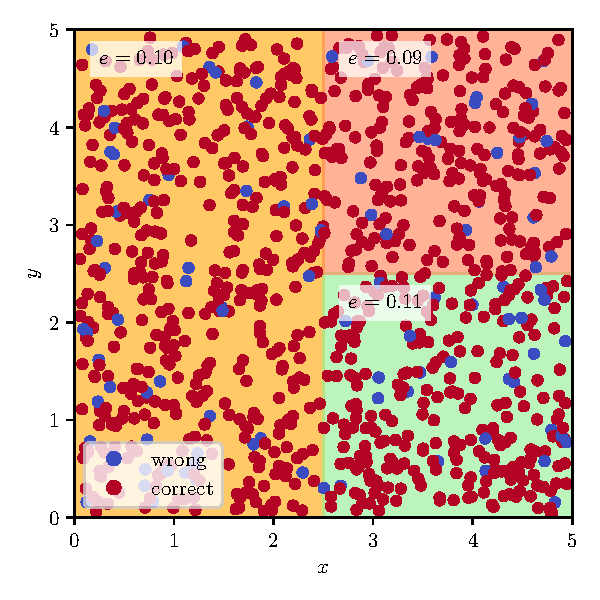
\includegraphics[width=0.295\linewidth]{figures/class-err.pdf}\label{fig:ge1}
	}
	\subfloat[Constant outputs.]{
		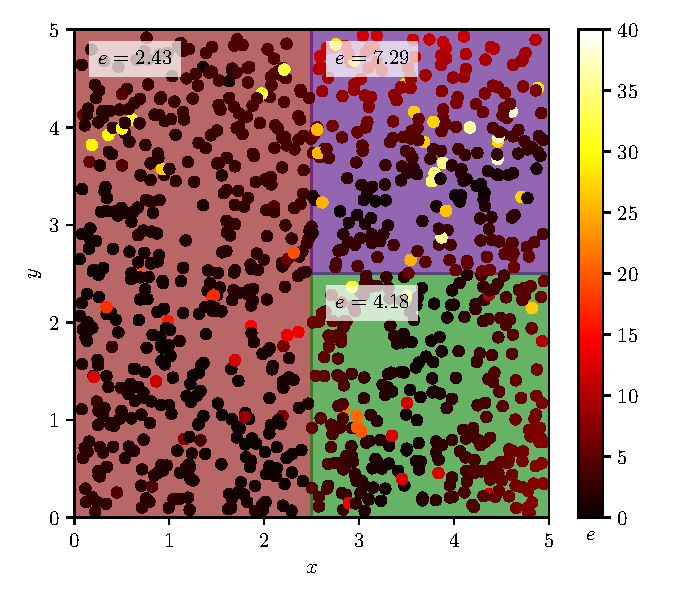
\includegraphics[width=0.34\linewidth]{figures/const-err.pdf}\label{fig:ge2}
	}
	\subfloat[Regression laws.]{
		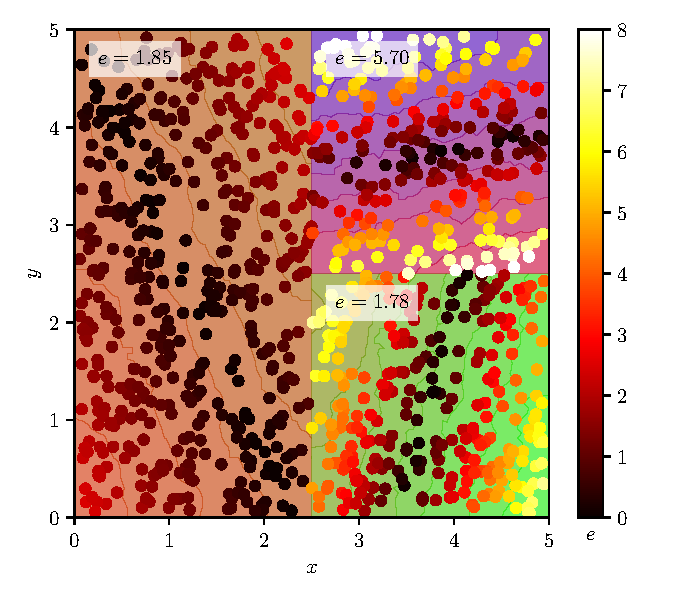
\includegraphics[width=0.34\linewidth]{figures/regr-err.pdf}\label{fig:ge3}
	}
	\caption{Two-dimensional example of different predictive errors measured for generalised extractors. Hatched regions are suitable to be merged with the adjacent one (coloured background).}\label{fig:general-error}
\end{figure*}
